\documentclass[12pt,a4paper]{article}
\usepackage{datetime}
\usepackage{hyperref}
\usepackage{graphicx}
\usepackage{color}
\usepackage{amsmath}
\usepackage{siunitx}

\begin{document}

\title{BOLODSP Software User's Guide}

\author{Jack Lovell\thanks{\texttt{jack.lovell@ukaea.uk}}}

\date{\today}

\maketitle

\abstract{This document serves as a guide for the end user to work with the BOLODSP software package which is bundled with D-TACQ's ACQ400 series firmware.
  A basic theory of operation is presented, and the parameters which control the operation of the BOLODSP module are discussed. General operation of
  D-TACQ's software, and the implementation details of the software and associated FPGA firmware module, are out of scope.}

\tableofcontents

\section{Introduction}
The BOLODSP software package is part of a custom module for D-TACQ ACQ400 series products used to operate the BOLO8BLF hardware module. It provides
software control of the BOLODSP FPGA module through a series of Linux commands, as well as some helper applications to simplify the fine tuning of the
signal processing capabilities of the module.

This document is \textit{not} a general user guide for D-TACQ software. For that, refer to the D-TACQ 4G user guide at \mbox{\url{http://www.d-tacq.com}}.
It is only concerned with the commands and settings provided by the package itself. Likewise, any requests for support with operating a system with this
package installed should be directed to D-TACQ directly, and not to the author, unless the query is specifically about an aspect of the BOLODSP module.

\section{Theory of Operation}
\subsection{Voltage Measurement}%
\label{sec:voltage}
\begin{figure}
  \centering
  % 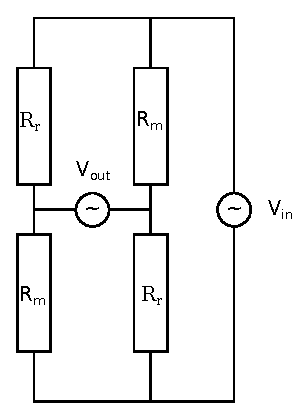
\includegraphics[width=0.3\textwidth]{sensor_schematic.eps}
  \def\svgwidth{0.3\columnwidth}
  \input{sensor_schematic.pdf_tex}
  \caption{Electrical schematic of bolometer sensor\label{fig:sensor}}
\end{figure}
A resistive bolometer consists of 4 resistors in a Wheatstone bridge configuration (see Figure~\ref{fig:sensor}), as described in Ref~\cite{mast-1991}.
The two resistors marked $R_m$ are ``measurement'' resistors, which are in thermal contact with a thin foil. Incident radiation heats the foil and hence
the resistors, increasing their resistance. The two resistors marked $R_r$ are ``reference'' resistors: they are not in contact with the foil, and so their
temperature (and hence resistance) remain constant.

When a voltage $V_{in}$ is applied across one diagonal of the bridge as shown, there will be zero output voltage $V_{out}$ if the bridge is balanced.
However, if the measurement resistors have increased resistance compared to the reference resistors, the bridge will be unbalanced, and $V_{out}$ will be
non-zero. By measuring $V_{out}$ it is therefore possible to calculate the resistance change of the foil, and by knowing the electrical and thermal
properties of the sensor it is possible to then infer the temperature change and the absorbed power. The details of these calculations are out of the
scope of this document.

To minimise noise in the system, AC synchronous detection is used to measure $V_{out}$. An AC excitation voltage $V_{in}$ is applied to the bridge,
typically a sinusoid with a frequency of a few 10s of kHz. The amplitude of $V_{out}$ at the same frequency is measured, and this voltage amplitude is
used in the bolometer equation to determine the absorbed power. The amplitude calculation (demodulation) is performed on the FPGA module, as follows.

The excitation voltage $V_{in}$ is of the form
\begin{equation}
  \label{equ:vin}
  V_{in} = V_0\sin(\omega t)
\end{equation}
Where $V_0$ is the amplitude of the excitation voltage and $\omega$ is the frequency. The output from the bridge due to the bridge imbalance is of the form:
\begin{equation}
  \label{equ:vout}
  V_{out} = A\sin(\omega t - \phi)
\end{equation}
Where the amplitude $A$ is the quantity we want to measure, and $\phi$ is the phase difference between the output and excitation voltages. This phase
shift is due to round trip time and parasitic capacitance in the system, and can be significant when there is a long cable between the electronics and
the sensor.

By multiplying $V_{out}$ with a normalised form of $V_{in}$ (which we shall call $V_{ref,i}$) and time averaging to remove the $2\omega$ frequency component
from the resulting signal, we can obtain the amplitude, assuming it varies slowly compared to the time averaging window. This is known as the ``in-phase''
component, since the signal is multiplied by a reference voltage of the same phase as the excitation voltage:
\begin{equation}
  \label{equ:I}
  \begin{split}
  I &= \frac{1}{n\pi}\int_{0}^{2n\pi}V_{ref,i}V_{out}\mathrm{d}\omega t \\
  &= \frac{1}{n\pi}\int_{0}^{2n\pi}\sin(\omega t) A \sin(\omega t - \phi)\mathrm{d}\omega t \\
  &= \frac{A}{2}\cos \phi
  \end{split}
\end{equation}
Equation~\ref{equ:I} still depends on the phase $\phi$. Traditionally, some phase shift has been applied to $V_{ref,i}$ such that $\phi = 0$ to remove the
phase dependence on $I$, but we employ a more general method. Consider a second reference, $V{ref,q}$ which is a quarter of a period out of phase with the
excitation voltage:
\begin{equation}
  \label{equ:Q}
  \begin{split}
  Q &= \frac{1}{n\pi}\int_{0}^{2n\pi}V_{ref,q}V_{out}\mathrm{d}\omega t \\
  &= \frac{1}{n\pi}\int_{0}^{2n\pi}\cos(\omega t) A \sin(\omega t - \phi)\mathrm{d}\omega t \\
  &= -\frac{A}{2}\sin \phi
  \end{split}
\end{equation}
We can now combine Equations~\ref{equ:I} and~\ref{equ:Q} to remove the phase dependence:
\begin{equation}
  \label{equ:A}
  A = 2\sqrt{I^2 + Q^2}
\end{equation}
Equation~\ref{equ:A} thus gives a measure of the amplitude of the output voltage independent of phase, and hence independent of the hardware used. This
method is known as ``quadrature detection''.

For completeness, the phase is given by:
\begin{equation}
  \label{equ:phi}
  \phi = -\tan^{-1}\left(\frac{Q}{I}\right)
\end{equation}

On the FPGA, the time averaging is done using a low-pass filter. The choice of filter coefficients will affect the integration time, or alternatively the
bandwidth of the output. Higher bandwidth allows higher time resolution, but comes at the cost of increased noise in the measurement, since higher
frequency noise components are less suppressed. A helper script exists to calculate the appropriate filter coefficients for a given bandwidth, and load
them onto the FPGA (see Section~\ref{sec:lpfdesign}).

The process of time averaging over multiple periods means it is no longer necessary to sample at a high enough rate to resolve the AC excitation
waveform. Instead, we only need to sample at a high enough rate to resolve amplitude (and phase) fluctuations below the cutoff frequency of the filter
used to perform the time averaging. Bolometer sensors naturally suppress high frequency signals due to the thermal properties of the sensor, so the
signal-to-noise ratio gets very low at higher frequencies. The BOLODSP module on the FPGA downsamples the output data by a factor of 100. This
means that for an input sampling rate of 1MSPS (the maximum sampling rate of the BOLO8BLF), data will be output at 10kSPS\@. This means that the FPGA
filters should be set to a maximum of 5kHz, though in practice there is little point going above about 1.5kHz.

\subsection{Voltage Offset}%
\label{sec:offset}
No sensor is perfect, in the sense that the bridge will never be perfectly balanced in the absence of any input power. Likewise, no electronics is perfect,
and there will always be some cross talk between excitation and measurement voltages. This leads to a voltage offset with no input power:
\begin{equation}
  \label{equ:voff}
  V_{off} = A_{off}e^{i\phi_{off}}
\end{equation}
Note that the offset voltage has both an amplitude \textit{and} phase, which may be different to the phase of the signal due to incident power, making the
measured voltage a complex signal. It is necessary to subtract this offset from the measured signal using a suitable complex subtraction, either by
decomposing into real ($I$) and imaginary ($Q$) parts and subtracting the real and imaginary parts of the offset respectively, or by performing a
vector-based subtraction using the cosine rule.

The FPGA firmware has the capability to perform the first of these methods on-chip, using user-loadable offset values for each channel
(Section~\ref{sec:offset_correction}). When offset subtraction has been correctly performed, the remaining phase should be constant (being only a property
of the geometry), and the remaining amplitude will be a measure only of the bridge imbalance (and hence the temperature change of the sensor foil). The
phase is therefore a useful measurement for data validation.

\subsection{Real-Time Power Output}%
\label{sec:rtpower}
The physics involved in calculating the power aborted by the foil from the resistance change of the meander resistors is complex, particularly when an AC
excitation voltage is involved. For a thorough treatment of the subject, see Ref~\cite{giannone-2002}. However, the following simplified formula gives a
good approximation of the more complex result:
\begin{equation}
  \label{equ:pbol}
  P = \frac{1}{S}\left(A + \tau \frac{\mathrm{d}A}{\mathrm{d}t}\right)
\end{equation}
Here, $S$ is the sensitivity of the sensor, and $\tau$ is the cooling time. Both these values can be calculated using an in-situ calibration procedure, as
described in Section~\ref{sec:calibration}.

The flexibility of the FPGA's digital filtering means it is possible to design a filter to both perform the time averaging described in
Section~\ref{sec:voltage}, and adding to this the time derivative as in Equation~\ref{equ:pbol}. Using this filter (known as a ``deconvolution'' filter)
will produce an estimate of the incident power straight from the bridge voltage measurement, with a latency of about 1ms, which should be quick enough to
use in a real-time control loop. The design of this filter requires an accurate calibration, and is discussed in Section~\ref{sec:calibration}.

\subsection{Calibration}%
\label{sec:calibration}
It can be seen from Equation~\ref{equ:pbol} that at least 2 quantities need to be determined from a calibration: the sensitivity $S$ and the cooling
time $\tau$. The sensitivity can be determined by measuring the change in the voltage output for a known input power, and the cooling time can be
calculated by fitting an exponential decay to the voltage curve as the sensor cools immediately after removing all input power. In the BOLO system,
the input power is provided by ohmic heating, by applying a DC bias (or offset) to both $V_{in}$ and $V_{out}$, whilst at the same time keeping the
AC excitation voltage of $V_{in}$ to simulate operation with radiation heating as closely as possible.

\begin{figure}
  \centering
  \def\svgwidth{\columnwidth}
  \input{calibration.pdf_tex}
  \caption{Electrical schematic of the calibration procedure\label{fig:calibration}}
\end{figure}

The calibration procedure is described in some detail in Ref~\cite{lovell-2015}. Figure~\ref{fig:calibration}, based on that paper, shows the calibration
procedure. The application of $V_{OS}$ is such that current flows through the two measurement resistors $R_M$, but not through the reference resistors
$R_R$. This causes only the measurement resistors to be ohmically heated, with the total heating power for both measurement resistors given by
\begin{equation}
  \label{equ:pohmic}
  P_{OH} = 2 V_{OS} I_{OS}
\end{equation}
Note that the voltages applied to the bridge are differential: the quantities $V_{AC}$ and $V_{OS}$ are those requested of the BOLO DACs, and $V_{OS}$ and
$I_{OS}$ are the quantities measured by the ADC.\@ The differential nature of the signal results in the signs and factors of 2 present in the voltages at
each point in the circuit.


When the ohmic heating is switched off, the sensor cools. The bridge voltage (amplitude and phase) measured during cooling provides a number of useful
calibration values. They must however be converted into Cartesian representation ($I$ and $Q$) first:
\begin{itemize}
\item{The offsets $A_{off}$ and $\phi_{off}$ can be calculated using Equations~\ref{equ:I} and~\ref{equ:Q}, using $I_{off} = I(t\rightarrow\infty)$ and
    $Q_{off} = Q(t\rightarrow\infty)$}
\item{The cooling time can be calculated by fitting an exponential decay of the $I$ and $Q$ cooling curves. The decay time constant is the cooling time.
    It should be the same (to within errors) for both curves.}
\item{The sensitivity is given by $S = \frac{P_{OH}}{\Delta A}$, where $P_{OH}$ is given by Equation~\ref{equ:pohmic} and $\Delta A$ is given by
    Equation~\ref{equ:A}, using $\Delta I = I(t=0) - I_{off}$, and $\Delta Q = Q(t=0) - Q_{off}$.}
\end{itemize}
During the calibration, the FPGA measures $V_{OS}$ and $I_{OS}$, in addition to $A$ and $\phi$, thus providing all the required data for a
calibration in one place. For consistency, we shall refer in the rest of this guide to $V_{OH}$ and $I_{OH}$, which are equal to $V_{OS}$ and
$I_{OS}$, to minimise confusion with the voltage offsets $I_{off}$ and $Q_{off}$ and the current measurement offset $I_{off}$ (see
Section~\ref{sec:scaling}).

\section{Data Outputs}%
\label{sec:outputs}
\subsection{Output Channel Format}%
\label{sec:channels}
For each physical channel on a BOLO8, there are 3 ``logical'' output channels. This means each BOLO8 site has 24 output channels, each of which can be read
like any other D-TACQ output (see the D-TACQ 4G user guide for details). All channels are 4-byte signed integers. The channels are arranged as follows:
\begin{enumerate}
\item{The voltage amplitude $A$ from the quadrature synchronous detection process (Section~\ref{sec:voltage}).}
\item{The phase $\phi$ from the quadrature synchronous detection process (Section~\ref{sec:voltage}).}
\item{The third channel depends on the operating mode:}
  \begin{enumerate}
  \item{During normal mode: the real-time power calculation from the deconvolution process (Section~\ref{sec:rtpower}).}
  \item{During calibration mode: a combination of the ohmic heating voltage $V_{OH}$ and current $I_{OH}$ (Section~\ref{sec:calibration}). The top 2 bytes of
      each 4-byte sample are the voltage, and the bottom 2 bytes are the current. In other words, this output is $V_{OH} \times 2^{16} + I_{OH}$. In this
      scenario, $V_{OH}$ is a signed 2-byte integer, and $I_{OH}$ is an unsigned 2-byte integer.}
  \end{enumerate}
\end{enumerate}

For a physical channel $N$ (numbered 1--8 per site), logical channel $3N-2$ is the voltage amplitude, $3N-1$ is the voltage phase and $3N$ is either the
real-time power or calibration quantities. So for example, for physical channel 3, logical channel 7 is the amplitude, 8 is the phase and 9 is
power/calibration signals.

\subsection{Data Scaling}%
\label{sec:scaling}
The following are the numerical conversion factors to convert from raw counts (the 2- or 4-byte values read from the device) into physical units. There is
a dependence on $V_{gain}$, which is the voltage gain used on the BOLO8's ADCs. The value can be read back as a knob in CSS or EPICS (or your favourite data
acquisition tool); contact D-TACQ for the details of setting and reading these values. The recommended gain is 1V2 (1.25V), since the bolometer signals are
typically small (10s to a few 100s of mV), even with strong radiation.

There is also a dependence on the CORDIC scale factor:
\begin{equation}
  \label{equ:cordic}
  \begin{split}
    Z_{30} &= \prod_{i=1}^{30}\sqrt{1 + 2^{-2i}} \\
    &= 1.1644353\ldots
  \end{split}
\end{equation}
This is due to the algorithm used to convert $I$ and $Q$ into $A$ and $\phi$ on the FPGA\@.

The scalings are as follows:
\begin{equation}
  \label{equ:avolts}
  \begin{split}
    A(V) &= A(counts) V_{gain} \frac{20}{18 \times 2^{24} \times Z_{30}} \\
    &= A(counts) V_{gain} \times 5.6875105\ldots \times 10^{-8}
  \end{split}
\end{equation}

\begin{equation}
  \label{equ:phirad}
  \begin{split}
    \phi(rad) &= \phi(counts) \times 2^{-29} \\
    &= \phi(counts) \times 1.8626451\ldots \times 10^{-9}
  \end{split}
\end{equation}

\begin{equation}
  \label{equ:pwatts}
  \begin{split}
    P(W) &= P(counts) V_{gain} \frac{20}{18 \times 2^{18} \times Z_{30}} \\
    &= P(counts) V_{gain} \times 3.6400067\ldots \times 10^{-6}
  \end{split}
\end{equation}

\begin{equation}
  \label{equ:vdcvolts}
  \begin{split}
    V_{OH}(V) &= V_{OH}(counts) V_{gain} \times 2^{-15} \\
    &= V_{OH} V_{gain} \times 3.0517578\ldots \times 10^{-5}
  \end{split}
\end{equation}

\begin{equation}
  \label{equ:curramps}
  \begin{split}
    I_{OH}(A) &= I_{OH}(counts) \times \frac{128}{100} \times \frac{25}{3 \times 2^{12} \times 1000} - I_{off} \\
    &= I_{OH}(counts) \times 2.6041666\ldots \times 10^{-6} - I_{off}
  \end{split}
\end{equation}

$I_{off}$ in Equation~\ref{equ:curramps} is the current reading when $V_{OH} = 0$, i.e.\ no bias voltage is applied. In theory it should be around
$20.83 \times 10^{-3} \mathrm{A}$ but will vary slightly between channels. The most reliable way to measure $I_{off}$ is to take the mean value of
the current during the cooling part of the calibration.

\section{Control Knobs}%
\label{sec:knobs}
This section describes the control knobs available for the BOLODSP module. They are read and set in the same way as standard D-TACQ knobs using the remote
command interface, with the BOLODSP module treated as Site 14. See the D-TACQ 4G user guide for details.

\subsection{Low-level knobs}%
\label{sec:knobsll}
These control knobs are a fairly low level interface to the underlying FPGA module. For the most part they will be set by utility scripts. The ones which
may require the user to manually set them (or at least write a script to do so during the shot cycle) are documented here.

\subsubsection{DSP{\_}RESET}
Set to 1 to reset the BOLODSP firmware module. Set to 0 to remove from reset. To ensure correct channel ordering and an accurate time base for the data,
the module should be reset before each acquisition (transient or streaming). To perform a reset, run the \mbox{\path{/usr/local/bin/reset.dsp}} command.

\subsubsection{STEP{\_}SIZE}
This is used to generate the AC excitation voltage to the sensor. The excitation voltage is a sine wave of 18V amplitude. Note that the electronics is
capable of $\pm 20\mathrm{V}$ output; the 2V headroom is left to enable DC biasing during calibration. Due to implementation details in the BOLODSP
module, the STEP{\textunderscore}SIZE value $S$ required to produce an excitation voltage of $f$ Hz is given by:
\begin{equation}
  \label{equ:step_size}
  S = \frac{f}{f_{clk}} \times 2^{27}
\end{equation}
Here, $f_{clk}$ is the system clock frequency. Is is typically 100 MHz on older D-TACQ systems, and 125 MHz on newer systems. Contact D-TACQ if you are
unsure which frequency to use (or pick one and check the output on a scope to see if it's the correct frequency).

There also exists a script, \mbox{\path{/usr/local/bin/set.fdrive}~\texttt{<freq>}}, which takes a frequency in Hz and automatically sets the register
correctly. By default it assumes 100 MHz system clock, but this can be changed by modifying the script contents (contact D-TACQ or the author for
details).

\subsubsection{CALIBRATION}
Set to 1 to put the device in calibration mode, 0 to put it in normal mode. This changes the data output in the third logical channel for each physical
channel (Section~\ref{sec:channels}). This is done automatically by the calibration script in Section~\ref{sec:run_calibration}.

\subsubsection{FILTER{\_}STATUS}
This is a read-only knob, and indicates the readiness of the filters on the FPGA to be reloaded. It reports a hexadecimal value, and should be
\texttt{0x33} before attempting any reload. If it reads anything else, ensure you have read back any previous capture data and then run %chktex 29
\mbox{\path{/usr/local/bin/wait_for_filters}}, which will do a short capture to pass data through the filters so they are ready for the next reload.

\subsection{High-level knobs}%
\label{sec:knobshl}
These control knobs interface with the BOLODSP module at a higher level. Their inputs are in physical units, rather than register settings, and the
utility scripts read these knobs in order to set the lower-level knobs. All high-level knobs presented by the BOLODSP package are described here, and
should be set by the user.

\subsubsection{DIODE{\_}DROP{\_}V}
This value, in volts, sets the extra voltage to apply to one diagonal of the bridge to compensate for the voltage drop across diodes in the electronics.

The electronics features some diodes for noise reduction. There will be a voltage drop across these diodes, meaning that the applied bias voltage $V_{OH}$
in calibration will be less than the requested voltage on one of the bridge diagonals. Set this knob (in volts) to apply an extra voltage across that
diagonal to compensate for the voltage drop. The value should be tweaked until the measured ohmic heating voltage $V_{OH}$ (Section~\ref{sec:channels}) is
close to that set by the VBIAS knob. As a guide, when VBIAS is set to 1V, the diode voltage drop is about 0.5V for a $1.2\mathrm{k}\Omega$ bolometer
sensor.

\subsubsection{FILTER{\_}BANDWIDTH}
As mentioned in Section~\ref{sec:voltage}, the choice of filter affects the trade-off between noise levels and time resolution. The filters themselves are
designed using helper scripts (Section~\ref{sec:lpfdesign}). Those scripts take the value of this knob to design a filter with a given bandwidth. The
bandwidth should be specified in Hz. The maximum supported bandwidth is 1950Hz for use with the filter helper scripts.

\subsubsection{THEAT}
This value, in seconds, specifies the length of time spent ohmically heating the sensor during calibration. It should be long enough to ensure the sensor
has reached equilibrium, i.e.~several cooling times.

\subsubsection{TCOOL}
This value, in seconds, specifies the length of time to continue measuring the calibration curve after ohmic heating is turned off. It thus controls the
amount of the cooling curve measured. Like with THEAT, it should be set to multiple cooling times such that the sensor is nearly back in thermal
equilibrium at the end of the measurement.

\subsubsection{VBIAS}
This value, in volts, specifies the bias voltage $V_{OH}$ to be used to ohmically heat the bridge during calibration. It must be $<1.2\mathrm{V}$. The
required setting for DIODE{\_}DROP{\_}V will typically depend upon this knob.

\subsubsection{CAL{\_}EN}
Set this to 1 to enable a calibration before a shot. You should ensure that the data acquisition system of which the unit is a part is set up to run 2
acquisitions during the shot cycle: one to acquire the calibration data and a second to acquire the shot data.

This knob is ignored by the BOLODSP module and software, but may be helpful for user-written shot-cycle scripts to examine and work out what they need to
do.

\subsubsection{CAL{\_}DELAY}
This value, in seconds, specifies the length of time to wait between the start of a shot cycle (i.e.~prepare/arm) and the start of a calibration
procedure. It allows the user to cause the calibration procedure to run at a known time in the shot initialisation sequence. This could for example mean
performing the calibration as close as possible to the start of the shot, for conditions as similar as possible during the calibration and shot, or
performing the calibration earlier before sources of electrical noise such as coil power supplies are switched on.

Like the CAL{\_}EN knob, this is ignored by the BOLODSP module and software, but exists to allow user-written shot-cycle scripts to examine it and work
out when they need to call the calibration script.

\section{Operation}%
\label{sec:operation}
This section documents the usage of the various helper scripts throughout a shot cycle. Before a shot, a calibration should be performed (possible before
every shot, but not strictly necessary), and the results of the calibration should be used to remove offsets from the signal and design the filters for
the voltage and power output. After every capture (shot or calibration run) the BOLODSP module should be reset, using the
\mbox{\path{/usr/local/bin/reset.dsp}} script, to ensure the correct channel ordering and to clean out any stale data from the signal processing
module.

Refer also to the data capture section of the D-TACQ 4G user guide for details of how to set up a transient capture.

\subsection{Calibration}%
\label{sec:run_calibration}
A calibration run proceeds as follows. These steps should be performed by a user-written script, perhaps as part of a shot cycle script.
\begin{enumerate}
\item{Set the high-level knobs described in Section~\ref{sec:knobshl}, and set the STEP{\_}SIZE low-level knob to give the desired excitation
    frequency.}
\item{Reset the DSP system, by running the \mbox{\path{/usr/local/bin/reset.dsp}} script. This ensures the channel ordering and time bases will be
    correct.}
\item{Set the offsets for all voltage channels to 0 (Section~\ref{sec:offset_correction})}.
\item{Set up a transient data capture, set to wait until the system receives soft trigger, to acquire at least $(0.1 + T_{HEAT} + T_{COOL})\times 10000$ samples. For example, if $T_{HEAT} = T_{COOL} = \SI{1}{s}$:\\
    \verb!set.site 0 `transient POST=21000 SOFT_TRIGGER=0; set_arm'!\\
    The system is now ready to perform the calibration.}
\item{Run the \mbox{\path{/usr/local/bin/bolo_calibration}} script, which controls the hardware to perform a calibration procedure, as described in
    Section~\ref{sec:calibration}. To run it, a user or script must have SSH access to the device. It reads the voltage and timing high-level knobs, and
    proceeds as follows:
\begin{enumerate}
\item{Put the device in calibration mode, so that $V_{OH}$ and $I_{OH}$ are recorded, instead of real-time power.}
\item{Trigger the data collection.}
\item{Wait 0.1 seconds to measure the voltages and current with no heating applied (this can be helpful in post-processing).}
\item{Turn the ohmic heating on, and wait for THEAT seconds}.
\item{Turn the ohmic heating off, and wait until data collection finishes.}
\item{Put the device in normal mode, so that the real-time power will be output on the next capture.}
\end{enumerate}
}
\item{Reset the DSP system again before the shot, to ensure the correct channel ordering and time base.}
\end{enumerate}

The capture data should be read back before the shot capture is started, as the latter will overwrite the calibration data with shot data. The procedure
takes THEAT + TCOOL + a few seconds to complete, plus the time to read back the calibration data. It is advisable to allow at least 30 seconds from
starting a calibration to the expected shot trigger, just in case, but the procedure is quick enough to be performed before every shot if needed. Of
course, a calibration can also be performed separately, by following this procedure manually.

\subsubsection{The calibfit utility}%
\label{sec:calibfit}
Newer versions of the BOLODSP package (those built after 16th December 2016) include the \mbox{\path{/usr/local/bin/calibfit}} command. This can be
called after a calibration run has been performed and the data captured with a transient capture, and will automatically perform curve fitting on the
data to calculate the sensitivity, cooling time and voltage offsets for a given channel. These can be used to load the offset registers
(Section~\ref{sec:offset_correction}) and design the deconvolution filters for the real-time power output (Section~\ref{sec:lpfdesign}) without having
to read the data from the device, calculate the fit parameters offline and then send the correct parameters back to the device.

The \texttt{calibfit} utility works on a single channel, supplied via a command line argument. Using $V_{OH}$ it determines what part of the time trace
is heating, and which part is cooling: if $V_{OH}$ is above a threshold value then the sensor is being ohmically heated at that time, and if it is
below a threshold value after a given time (to allow for the short pause for offset measurement at the start of the calibration) then it assumes
cooling is occurring. The utility thus requires that the calibration has been performed in the manner described in Section~\ref{sec:run_calibration},
preferably using the \texttt{bolo\_calibration} utility. The wait time and heating/cooling thresholds are configurable as command line parameters.

From the heating phase, \texttt{calibfit} calculates the applied ohmic heating power using $P_{OH} = 2 V_{OH} I_{OH}$, which is used in the sensitivity
calculation. From the cooling phase, it calculates $I$ and $Q$ using Equations~\ref{equ:I} and~\ref{equ:Q} and then fits the following curve (same
for $Q$):
\begin{equation}
  \label{equ:Icool}
  I_{cool} = \Delta I e^{-t / \tau} + I_{off}
\end{equation}
Here, $t$ is the time since cooling started, and $\Delta I$, $\tau$ and $I_{off}$ are the fit parameters (for performance reasons $1/\tau$ is fitted,
but the program outputs $\tau$). To generate the time vector $t$ for the fit, the program assumes a sample rate of 10kSPS, which is the expected output
sample rate if setting the BOLO8s to sample at 1MSPS\@.

The sensitivity is calculated from $\Delta I$, $\Delta Q$ and $P_{OH}$ as described in Section~\ref{sec:calibration}. The cooling time is the average
of the $I$ and $Q$ fits, since the cooling time is independent of the phase (and therefore should be identical for both $I$ and $Q$ fits if the fits
were perfect and free of noise). The offsets $A_{off}$ and $\phi_{off}$ are calculated from $I_{off}$ and $Q_{off}$ using Equations~\ref{equ:I}
and~\ref{equ:Q}, though both polar and Cartesian offsets are output by the utility, so offset correction can be done either on-chip
(Section~\ref{sec:offset_correction}) or in post-processing using the user's preferred method (see Section~\ref{sec:offset}).

The \texttt{calibfit} utility takes the following command line options:
\begin{verbatim}
calibfit [-c channel] [-C cooling_theshold]
         [-H heating_threshold] [-t t_wait] [-T tau_guess]
\end{verbatim}
The options are as follows:
\begin{itemize}
\item{\texttt{channel}: The physical channel to use. Default=1}
\item{\texttt{cooling\_threshold}: Assume cooling if the voltage is below this threshold (in V), and after t\_wait. Default=0.001}
\item{\texttt{heating\_threshold}: Assume heating if the voltage is above this threshold (in V). Default=0.95}
\item{\texttt{t\_wait}: Assume no cooling occurs before this time (in seconds). Default=0.2}
\item{\texttt{tau\_guess}: Initial guess at the cooling time (in seconds), to aid the fit. Default=0.2}
\end{itemize}

A sample output of the program is below, done for a calibration of a sensor in air:
\begin{verbatim}
acq2106_006> calibfit -c13
Successfully read 21000 samples
Fit parameters for i: 0.003383145	16.24632	-0.02794252
Fit parameters for q: -0.003408019	16.20701	0.02941226
Fitting complete. Fit parameters:
sens = 6.098115
tau = 0.06162704
a0 = 0.08113854
phi0 = -2.330575
i0 = -0.02794252
q0 = 0.02941225
\end{verbatim}
The output is printed to \texttt{stdout}. It is the user's responsibility to redirect the output to a file to record for posterity, and/or parse the
output to have the device automatically load the offset registers (Section~\ref{sec:offset_correction}) and the real-time power filter
(Section~\ref{sec:lpfdesign}).

\subsubsection{Example calibration data}%
\label{sec:example-calibr-data}

We have provided screen grabs of the 3 calibration traces, shown in CSS using the plot transient tab, to give an example of what a successful calibration of a bolometer sensor should look like.
Note that the precise values will vary significantly with different hardware.
In particular, the phase values will change with cable length, and if the phase is positive then the amplitude signal will look like it is inverted compared to these examples.
Successful offset subtraction (see Section~\ref{sec:offset} and Section~\ref{sec:offset_correction}) will correct for this.

Figure~\ref{fig:example-acal} shows the voltage amplitude, without any offset correction applied.
Figure~\ref{fig:example-phical} shows the phase, again without any offset correction.
Figure~\ref{fig:example-dc} shows the DC channel, which contains both the DC bias voltage and the current applied to the bridge in the form $V_{DC} \cdot 2^{16} + I_{DC}$.

\begin{figure}
  \centering
  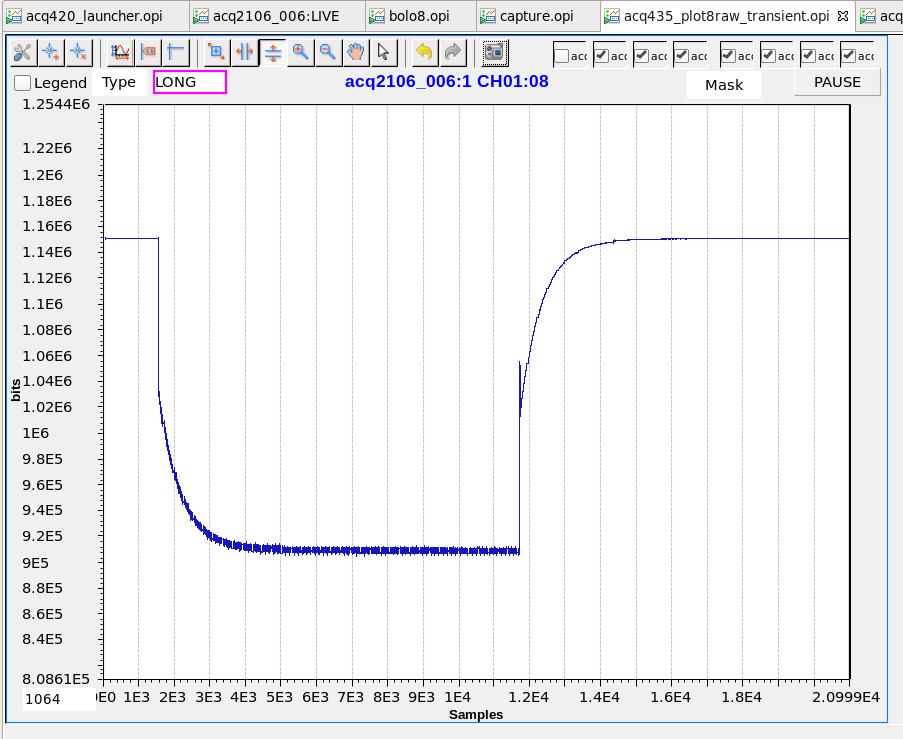
\includegraphics[width=\textwidth]{acal_CSS.png}
  \caption[Example trace for the bridge amplitude for a calibration]{Example trace for the bridge amplitude for a calibration.
    There are 3 regions: the first 1.5E3 samples with no heating indicates the amplitude offset.
    Then there are approximately 1E4 samples of heating, where the bridge heats up (shown an an exponential curve) as the DC bias voltage is applied.
    Finally, the last 1E4 samples show the cooling curve: the exponential decay of the bridge amplitude as the measurement resistors return to equilibrium.
    Note that the signal appears to be inverted here (an increase in the bridge temperature reduces the amplitude), but this is simply due to the phase being negative.
    After performing offset correction this particular trace will be inverted, and the first 1.5E3 samples will be approximately 0.
    Different cabling setups affect the phase, so this trace may or may not be inverted for other users (though whether or not a given channel is inverted should be the same across successive calibrations if the hardware arrangement remains the same).\label{fig:example-acal}}
\end{figure}

\begin{figure}
  \centering
  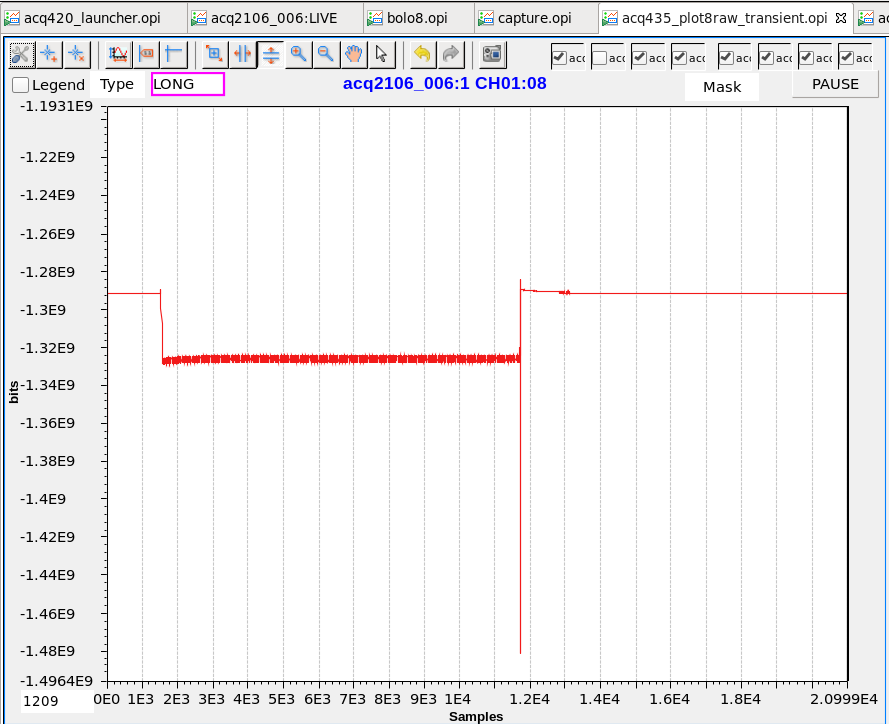
\includegraphics[width=\textwidth]{phical_CSS.png}
  \caption[Example trace for the phase for a calibration]{Example trace for the phase for a calibration.
    The phase changes relatively little, though there is a noticable different between heating and cooling due to the internal hardware of the BOLO8 board.
    Note that the phase in this case is negative, which causes the amplitude  trace to be inverted: it may not be in other setups with different cabling.\label{fig:example-phical}}
\end{figure}

\begin{figure}
  \centering
  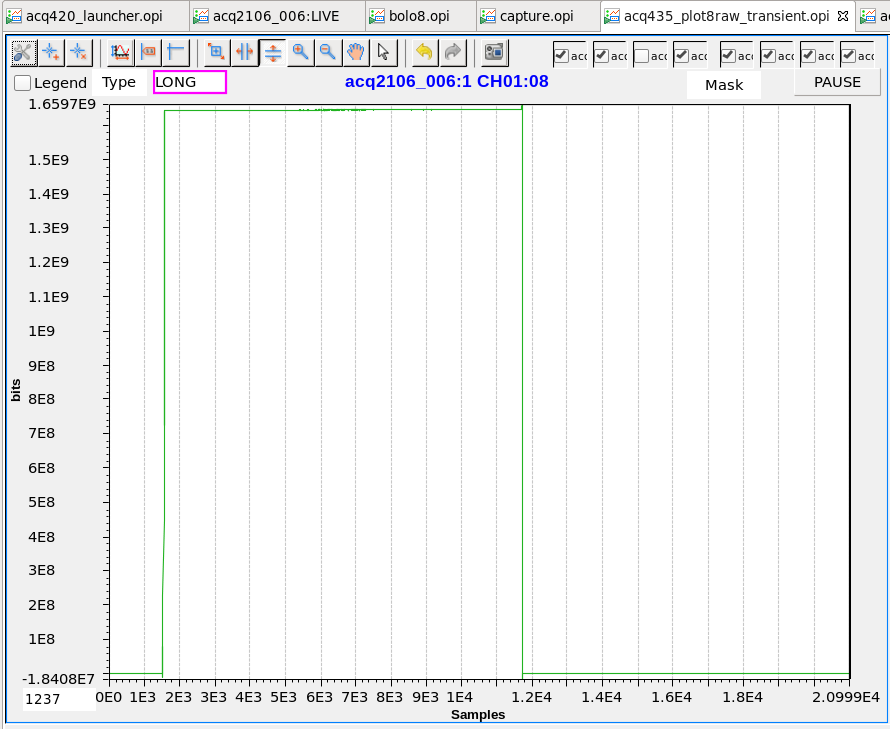
\includegraphics[width=\textwidth]{VDC_CSS.png}
  \caption[Example trace for the DC bias in a calibration]{Example trace for the DC bias in a calibration.
    This includes both the DC bias voltage and the current flowing through the resistors.
    The initial 1.5E3 samples with no heating, the 1E4 samples of heating and the 1e4 samples of cooling can clearly be seen.
    Since this quantity is actually $V_{DC} \cdot 2^{16} + I_{DC}$, even a small negative voltage during the cooling will appear to produce a large negative quantity in CSS.\@
    In this case, the heating voltage was \SI{1}{V}, and during cooling \SI{0.01}{V} was measured.
    The current measurement, being $2^{16}$ times smaller than the voltage measurement, is impossible to see.\label{fig:example-dc}}
\end{figure}

\subsection{Offset Correction}%
\label{sec:offset_correction}
As described in Section~\ref{sec:offset}, the voltage measured by the BOLO8 will include an offset due to intrinsic bridge imbalance and cross talk in the
electronics hardware and cabling. The offset can be measured from a calibration, either from the initial 0.1s equilibrium method or the asymptotic voltage
calculated from the cooling curve --- both measurements should be equal. It is possible to remove this offset in post processing, but the BOLODSP FPGA
module also has the ability to remove it during on-chip processing. This is particularly necessary for the real-time power signals if they are to be used
in a control loop, since no phase information is kept.

The on-chip offset correction consists of a series of registers which contain the $I_{off}$ and $Q_{off}$ values for each channel, followed by a second
series of registers which contain $P_{I,off}$ and $P_{Q,off}$ values, where $P_{I,off} = I_{off}/S$ and $P_{Q,off} = Q_{off}/S$ are the offsets in the
real-time power signals. The script \mbox{\path{/usr/local/bin/load_offset_channel.tcl}} can be used to load these registers for a particular channel. It
takes 4 mandatory arguments:
\begin{enumerate}
\item{\texttt{channel}: the channel to load, numbered from 1 to 48 (8 channels per site).}
\item{\texttt{I0}: the offset value $I_{off}$ in V.}
\item{\texttt{Q0}: the offset value $Q_{off}$ in V.}
\item{\texttt{sens}: the sensitivity, as described in Section~\ref{sec:calibration}, in V/W.}
\end{enumerate}

The offsets can be loaded at any time, including just before a shot. This is important, as the offset measured in a calibration long before a shot may not
be exactly equal to the offset when the machine is running with a full complement of power supplies and magnetic fields potentially affecting the sensor
and cabling. The neutral gas pressure may also affect the offset. Accurately predicting the offset drift throughout a shot cycle is an interesting area of
research~\cite{zhang-2012}.

\subsection{Filter Design}%
\label{sec:lpfdesign}
As described in Section~\ref{sec:voltage}, the calculation of the voltage amplitude and phase involves time averaging, which is performed on the D-TACQ
unit with a low-pass filter. In addition, the real-time power calculation uses a deconvolution filter, as described in Section~\ref{sec:rtpower}. The
bandwidth for both of these filters is set using the FILTER{\_}BANDWIDTH control knob (Section~\ref{sec:knobshl}).

The filter used to calculate the voltage is designed and loaded onto the FPGA by the \mbox{\path{/usr/local/bin/lpfdesign.tcl}} script. It takes no
arguments, and loads a single filter which is used by all channels.

The deconvolution filter used to calculate the power is designed and loaded by the \mbox{\path{/usr/local/bin/power_filter_design.tcl}} script. It takes 3
arguments:
\begin{enumerate}
\item{\texttt{channel}: the channel to load, numbered from 1 to 48 (8 channels per site).}
\item{\texttt{sens}: the sensitivity of the channel as calculated from a calibration, in V/W.}
\item{\texttt{tau}: the cooling time for the channel as calculated from a calibration, in seconds.}
\end{enumerate}
Since each channel will have different calibration factors, a different deconvolution filter must be loaded for every channel being used. Including the
sensitivity in the filter design allows the same scaling factor (Equation~\ref{equ:pwatts}) to be applied to every channel to convert to physical units
afterwards. When loading a new deconvolution filter, you should also update the offsets (Section~\ref{sec:offset_correction}) for that channel to
match. Like with the voltage filter, all deconvolution filters will have the same bandwidth, given by the control knob.

\textbf{Important}: between each deconvolution filter channel reload you \textbf{must} run \mbox{\path{/usr/local/bin/wait_for_filters}}, as described in
the FILTER{\_}STATUS knob in Section~\ref{sec:knobsll}. Failure to do so will lock up the system and require a hard reset.

\section{Conclusion}
This document describes the theory behind the BOLODSP module, which is intended to complement the D-TACQ BOLO8 hardware module. It also describes the
various settings and scripts used to operate the unit as a useful bolometer electronics back-end. For more detailed information about the system, consult
the references.

Finally, this is a very new product. There are likely to be bugs or undesirable ``features'', as in every new product (and indeed some very established
products). The source code for the software (and soon the FPGA firmware module) is freely available, and offers of collaboration for fixes or enhancements
will be warmly received.

\bibliographystyle{ieeetr}
\bibliography{refs}


\end{document}
